% !TEX root = ../main.tex
\section{Phân tích lỗi}\label{sec:error}

\subsection{Nghiên cứu tình huống: biển \code{54-L1 9999}}
Hình~\ref{fig:case} là một ảnh thật mà hệ thống đọc sai thành \code{5HL19999}. Kiểm tra từng bước cho thấy:

\begin{table}[H]
\centering
\caption{Lần theo lỗi qua từng bước của pipeline.}
\label{tab:case}
\begin{tabularx}{\linewidth}{lXl}
\toprule
Bước & Kết quả & Đánh giá \\
\midrule
Phát hiện & khung bao trọn biển, độ tin cậy 0,85 & đúng \\
Phân loại số dòng & 2 dòng & đúng \\
Tách dòng & \code{54-L1} và \code{9999}, ảnh sạch & đúng \\
CRNN, dòng 1 & \code{5HL1} (đáp án \code{54L1}) & \textbf{sai}: \code{4}$\to$\code{H} \\
Hậu xử lý & không khớp mẫu nào nên biển bị đánh dấu không hợp lệ & không cứu được \\
\bottomrule
\end{tabularx}
\end{table}

\begin{figure}[H]
\centering
\begin{subfigure}[b]{0.48\linewidth}
  \centering
  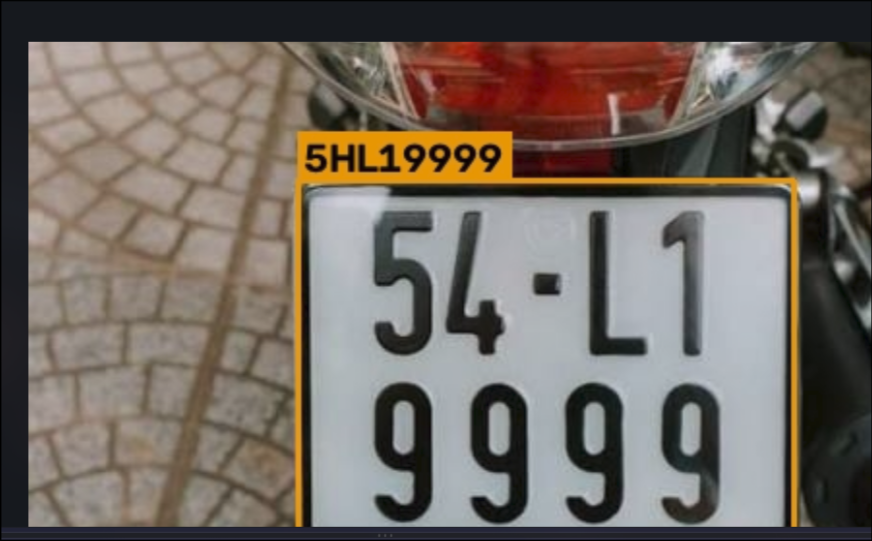
\includegraphics[width=\linewidth]{figures/case_54L1.png}
  \caption{Kết quả trên giao diện.}
\end{subfigure}\hfill
\begin{subfigure}[b]{0.48\linewidth}
  \centering
  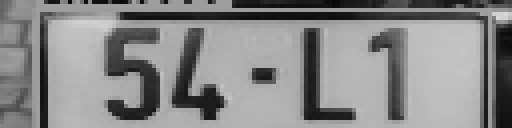
\includegraphics[width=\linewidth]{figures/case_line1.png}\\[0.4em]
  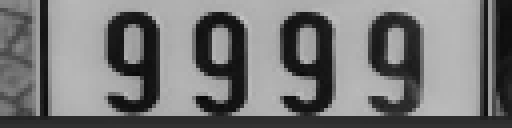
\includegraphics[width=\linewidth]{figures/case_line2.png}
  \caption{Hai ảnh dòng chữ CRNN nhận được ($32\times128$, phóng to).}
\end{subfigure}
\caption{Tình huống lỗi \code{54-L1 9999} $\to$ \code{5HL19999}.}
\label{fig:case}
\end{figure}

\paragraph{Nguyên nhân.} Lỗi nằm hoàn toàn ở CRNN, và gốc rễ là \textbf{khoảng cách miền} giữa dữ liệu tổng hợp và dữ liệu thật. Trong font Hershey dùng để sinh dữ liệu, số \code{4} có đỉnh khép kín. Trong font biển số Việt Nam, số \code{4} hở đỉnh, gồm hai nét dọc nối bằng một gạch ngang, nên hình dạng rất gần chữ \code{H}. Mô hình chưa từng thấy kiểu \code{4} này nên chọn chữ gần nhất trong những gì đã học.

Hậu xử lý cũng không sửa được, vì bảng \code{TO\_DIGIT} chỉ chứa các cặp nhầm phổ biến trong font Latin (\code{O}$\to$\code{0}, \code{B}$\to$\code{8}, \ldots), không có cặp \code{H}$\to$\code{4}, một cặp chỉ xuất hiện với font biển Việt Nam.

\subsection{Nhận xét chung}
\begin{itemize}[nosep]
  \item Bộ phát hiện và khối tiền xử lý hoạt động tốt trên ảnh thật. Điểm nghẽn của hệ thống là bộ nhận dạng.
  \item Độ chính xác trên dữ liệu tổng hợp (Bảng~\ref{tab:synth}) \emph{không} phản ánh độ chính xác trên biển thật. Đánh giá end-to-end trên dữ liệu thật là bắt buộc.
  \item Thiết kế hậu xử lý theo mẫu vẫn hợp lý, nhưng bảng nhầm lẫn nên được xây dựng từ lỗi thực tế (tệp \code{outputs/errors\_*.csv}) thay vì chỉ dựa trên trực giác.
\end{itemize}
